The Aggregator produces the Power model's final predictions for an entity by merging the Texter's and Ruler's predictions. As part of the merge process, the combined predictions are again sorted by confidence, increasing the density of true top predictions. Facts predicted by both, Texter and Ruler, are ranked especially high. However, although a predicted fact's confidence $conf_{Texter}$ assigned by the Texter and the confidence $conf_{Ruler}$ predicted by the Ruler are both from range $(0, 1)$, they are not necessarily directly comparable. As an example, an overconfident Texter might systematically assign too high confidences, while the Ruler is too pessimistic about its predictions, due to missing rules. Therefore, the Aggregator weights both component's decisions according to their credibility, yielding the decisive confidence $conf_{Aggregator}$ as per Equation~\ref{eq:4_approach/3_aggregator/conf_aggregator}.

\begin{align}
    conf_{Aggregator} = \alpha \cdot conf_{Texter} + (1 - \alpha) \cdot conf_{Ruler}
    \label{eq:4_approach/3_aggregator/conf_aggregator}
\end{align}

\begin{figure}[t]
    \centering
    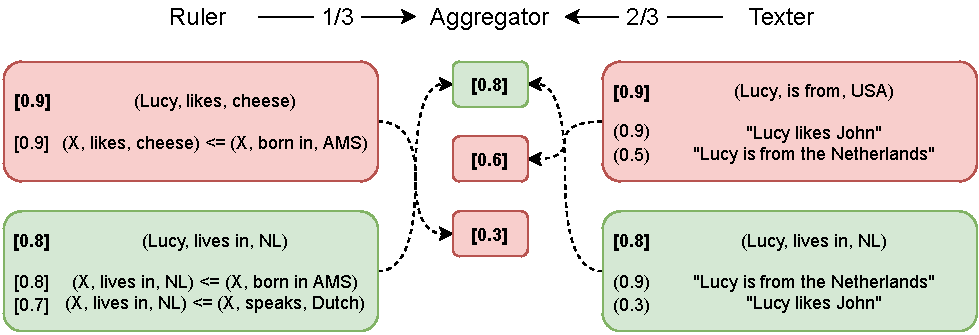
\includegraphics{4_approach/3_aggregator/lucy}
    \caption{The Aggregator merging the Ruler's and Texter's predictions whereby the Texter's predictions weight heavier for $\alpha = 2/3$ and facts predicted by both components rank the highest; Green/red indicate true/false positives, [brackets] mark confidences and (parantheses) mark attention values}
    \label{fig:4_approach/3_aggregator/lucy}
\end{figure}

To illustrate the function of the aggregator and recapitulate the Power model's overall approach, Figure~\ref{fig:4_approach/3_aggregator/lucy} demonstrates the inference process by an extended example based on the entity Lucy mentioned in the introductory example in Chapter~\ref{ch:1_introduction}. Concerning Lucy, we were given the sentences "Lucy is from the Netherlands." and "Lucy likes John." as well as the fact that Lucy was born in Amsterdam. In addition, it shall now be known, that Lucy speaks Dutch. As in the introduction, the aim is to predict the missig fact $(Lucy, lives~in, Netherlands)$. In this example scenario, calling the Ruler does indeed predict that with a probability of 80\%, since that is the confidence of the strongest rule. Unfortunately, however, the hypothetical graph seems to indicate that 90\% of all individuals born in Amsterdam also like cheese, resulting in an even higher ranked false positive, leading to precision = 0.5, recall = 1.0, F1 = 0.5 and mAP = 0.5. The situation is similar for the Texter: Again, the explanations for the predicted facts make sense, but the correct fact is only in second place. Regarding the predictions' confidence values, it should be noted that these do not result as the mean or maximum from the sentences' attention values. The latter are used exclusively for prioritization between sentences. Next, given the Ruler's and Texter's predictions, the Aggregator produces the final predictions in which the correct prediction moves to the first position, and although precision, and thereby F1, decrease to $\frac{1}{3}$ due to the coincidence of the true positives, the ultimately decisive mAP increases to 1.0. As noted at the top of Figure~\ref{fig:4_approach/3_aggregator/lucy}, the weight factor $\alpha$ corresponds to a scenario in which there are two correct Texter predictions for each Ruler prediction, which is of course exaggerated and serves the simple numbers. Furthermore, although left out in the figure, the aggregator predictions still include the explanations provided by Ruler and Texter.

% TODO Zwar liefern beide Komponenten Konfidenzen aus dem Bereich X, doch das bedeutet nicht zwingend dass eine 80 Vorhersage des Rulers gleichbedeutend mit einer 80 Aussage des Texters ist. Beispielsweise können bei einem zu kurz trainierten Ruler unbekannte Regeln dazu führen, dass die Abschätzung des Rulers systematisch zu niedrig ausfällt. Um zu verhindern, dass in diesem Fall eigentlich gute Vorhersagen hinter weniger guten Vorhersagen des Texters anstehen wird der Parameter alpha genutzt der zur Gewichtung der Vorhersagen von Ruler und Texter gemäß Gleichung Y genutzt wird. Darüber ob der Wert von alpha bei den evaluierten Daten nahe bei 5 liegt oder eher gegen Ruler oder Texter tendiert gab es bloß die oben erwähnte Vermutung, dass der Ruler systematisch unterschätzen könnte, was zu einer höheren Gewichtung des Rulers, also einem alpha kleiner 0,5 führen sollte.
